\chapter{Production 1}

\section{The beginning of the production}
    Due to this being the first production, three initial concepts will be made, based on research in the state of the art, that is separated into three different categories of experiences; gamified experiences, infographically driven experiences and indirectly informative experiences. These categories are derived from a combination of Copenhagen Zoo's wishes(as described in \autoref{problemArea}) for a final product and the research carried out in the analysis based on the initial problem statement (see \autoref{sec:ips}).
    
    % Hej Daniel :) vi skal lige snakke om dette afsnit :) - Sofie
    % - idea aspects (game/info graphics/indirect informative experiences) 
    % -Refere to analysis sections ( game elements, tech, Zoo wants a informative installation - info graphics.  

\section{State of the Art}
    The following section is a gathering of projects that uses the technology found in \autoref{Tech}, separated into three categories. These projects will work as inspiration for the design of the initial ideas in this production.
    
    \subsection{Infographically driven experiences}
    
	    \subsubsection{Augmented Reality Sandbox} % info graphics?
    	    This project is an augmented reality sandbox that dynamically visualized the depth of manipulated sand using a topological map, as well as a water flow model, was used in an introductory course for geology students. With an overwhelmingly positive response with students being helped in their understanding of the topic as well as preferring the artifact to traditional topological map exercises, being particularly useful to prevent misconceptions \cite{woods2016pilot}.
    
    	    The box was created with a real box of sand, a 3d scanning camera - a Microsoft Kinect, \todo{which can be seen in section XYZ,} visualization software, and a projector.  The sandbox can be seen in \autoref{fig:augmentedrealitysandbox}.
	    	\begin{figure}[H]
        		\centering
        		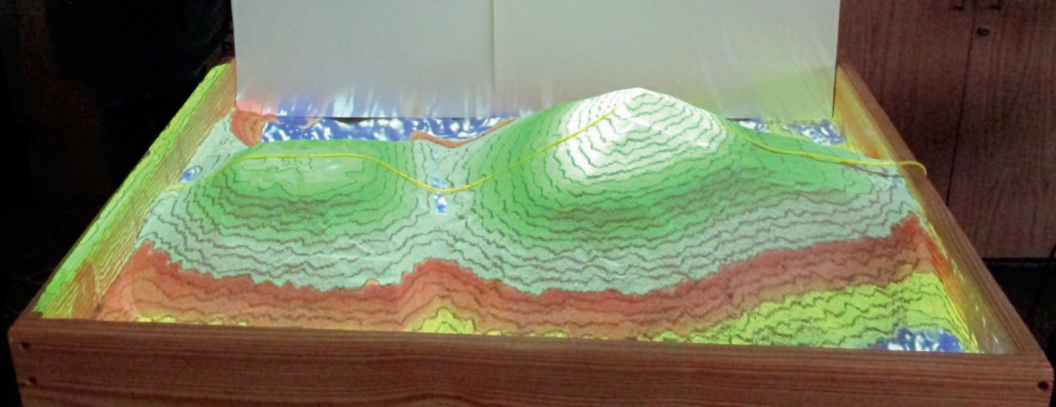
\includegraphics[width=0.9\linewidth]{figure/Analysis/augmentedrealitysandbox.png}
        		\caption{Augmented reality sandbox showing a topographical map of the sand. Simulated water can be seen on the other side of the hill \cite{woods2016pilot}.}
        		\label{fig:augmentedrealitysandbox}
        	\end{figure}
	    
	    \subsubsection{Interactive display at "The Blue Planet"} % indirect experience 
            The Blue Planet is an aquarium located in Copenhagen, Denmark. It's a new and modern facility, with several digital interactive installations. One installation is designed to make the users be the current of the ocean. Projectors show micro organisms on a wall and a Microsoft Kinect detects movement from users. As users walk by the wall, the shadow of the users pushes the micro organisms away from themselves, making the display behave according to the movement of the users.\cite{DenBlaPlanet} 
	

	
	\subsubsection{Transcending Boundaries}\label{sec:transcendingBoundaries} % experience
        Transcending Boundaries is an exhibition that ran in the beginning of 2017 at the Pace Gallery in London. It featured a series of immersive installations made by teamLab in an attempt to transcend the boundaries between digital artwork and the physical world\cite{transcendingBoundries}. \autoref{fig:transcendingBoundaries} shows a virtual waterfall, flowers and butterflies that are projected up on the walls and on the floor in one of the rooms of the exhibit using multiple projectors. The vegetation would indicate changes in seasons and would go through all 4 seasons every hour. Viewers in the room would obstruct the flow of water based on where they were standing and thereby became a part of the artwork.

        \begin{figure}[H]
        	\centering
        	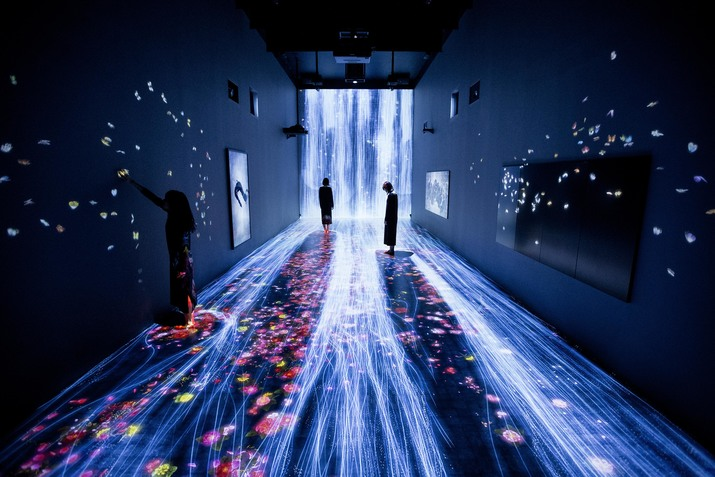
\includegraphics[width=0.9\linewidth]{figure/Analysis/transcendingBoundaries.jpg}
        	\caption{Figure showing 3 people interacting with the virtual waterfall installation from teamLab's exhibition at the Pace Gallery in London\cite{transcendingBoundries}.}
        	\label{fig:transcendingBoundaries}
        \end{figure}
  
        \subsubsection{INDE BroadcastAR} % experience
            INDE is a company that develops interactive augmented reality experiences using computer vision for entertainment-, educational- and inspirational purposes\cite{indeBroadcastAR}. The BroadcastAR system uses large screens placed on various public locations to attract and engage people that find themselves on screen in a 3D environment with photo-realistic 3D animals or people that react to their behavior without the use of any other devices (See \autoref{fig:indeBroadcastAR}).

            \begin{figure}[H]
            	\centering
            	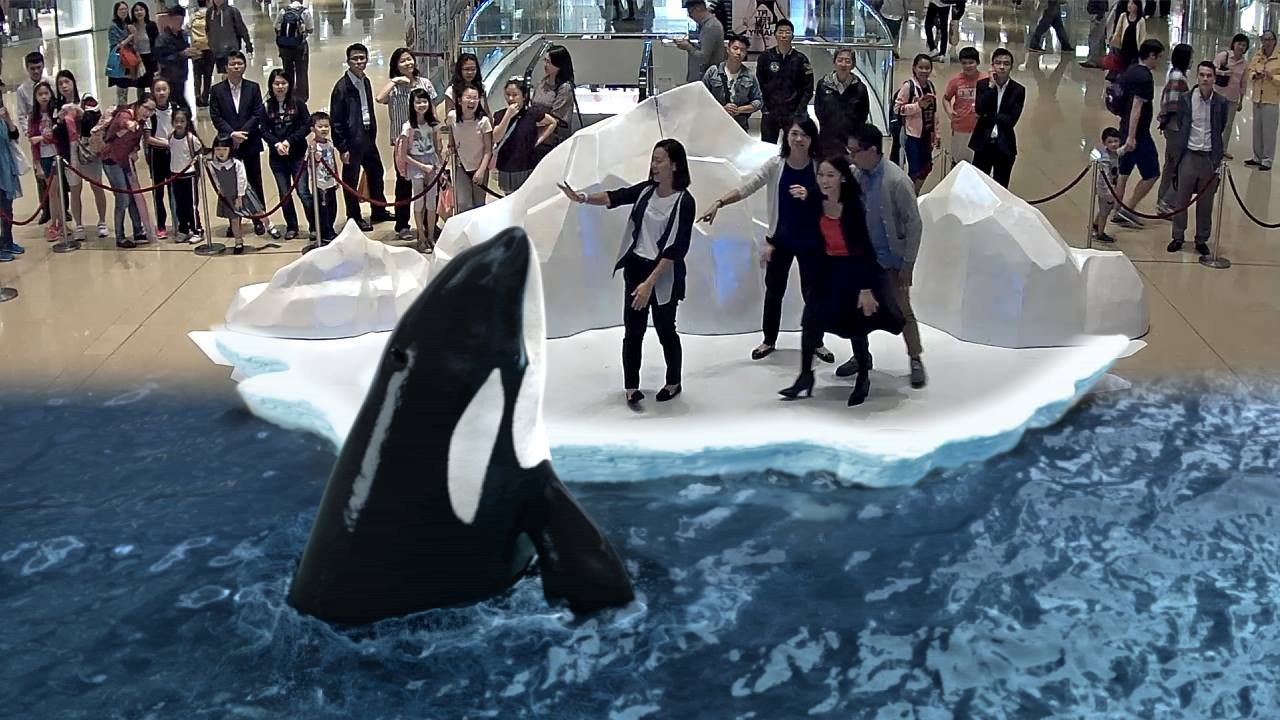
\includegraphics[width=0.9\linewidth]{figure/Analysis/inde.jpg}
            	\caption{The INDE BroadcastAR system put up in a mall. The images shows a digital 3D killer whale reacting to people on a platform resembling an arctic environment\cite{indeBroadcastAR}.}
            	\label{fig:indeBroadcastAR}
            \end{figure}

    \subsection{Gamified experiences}
        \subsubsection{Immersive Holodeck}\label{sec:leapMotionHolodeck} % category ?? game/info G/ experience
            A university in Ohio made an immersive \textit{"holodeck"} like experience, using 3 projectors in combination with a Leap Motion positioned in the the middle of the room. Using the leap motion, a user could manipulate objects in minecraft, like seen in \autoref{fig:holodeck}, or navigate around the world using Google maps\cite{leapMotionHolodeck}.
            
            \begin{figure}[H]
            	\centering
            	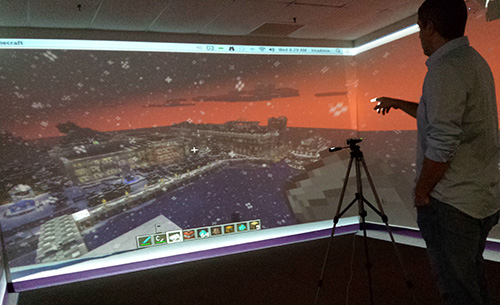
\includegraphics[width=0.7\linewidth]{figure/Analysis/holodeck.jpg}
            	\caption{Ohio university made immersive holodeck, made for immersive language learning\cite{leapMotionHolodeck}.}
            	\label{fig:holodeck}
            \end{figure}
            
            The purpose of the system, was to allow immersion while learning a language, putting you in the environments that the language is spoken.
    
        	\subsubsection{Interactive Projection Mapping Prototype} % Game?
    	    This project demonstrates the possibilities of manipulating the physical world using the Leap Motion in combination with an Arduino, as seen in \autoref{fig:leapProjector}. Using the Leap Motion API \todo{as described in section XYZ}, the creator allowed for simple gestures to control the box and pick up the pets in the world. The goal of the game is as simple as picking up the four pets and putting them on their pillow, all while rotating the cube to cycle through the different seasons and sides of the cube\cite{leapMotionProjectionMapping}.
    	    \begin{figure}[H]
    	    	\centering
    	    	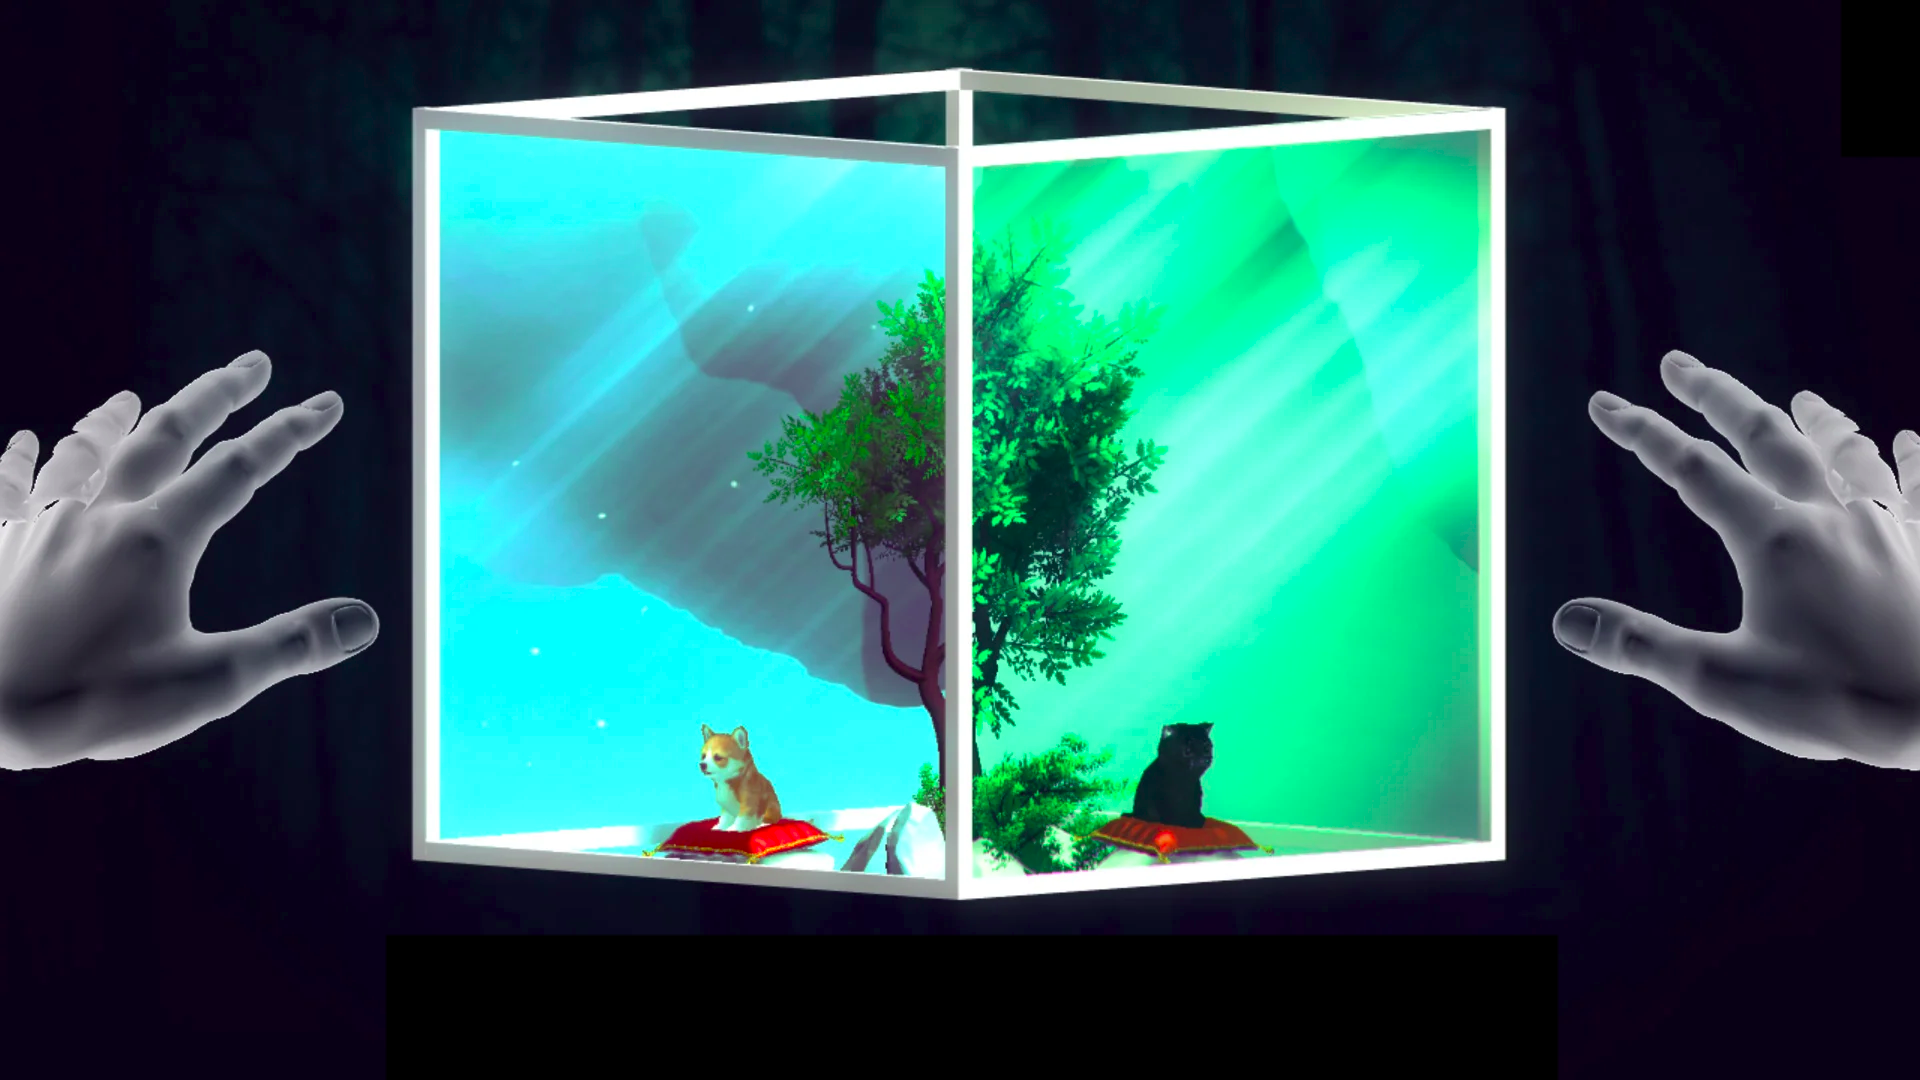
\includegraphics[width=0.8\linewidth]{figure/Analysis/LeapProjector.png}
    	    	\caption{A physical game, using the Leap Motion to pick up pets and rotating the physical cube using gestures\cite{leapMotionProjectionMapping}.}
    	    	\label{fig:leapProjector}
    	    \end{figure}
            The game can be played exclusively on the PC, without the physical cube. But the point from the creator's side was to learn to interface with the physical cube using the Leap Motion.


\section{Design}
To explore possible directions for the informative aspect, as well as these mentioned different approaches for conveying information though experiences, namely through gamified experiences, info graphically driven experiences and indirectly informative experiences, it was decided to design, implement and test three different initial concepts, each developed based on one of the mentioned approaches.

\subsection{Gamified experience concept - \textit{Feed a Penguin}}
The first prototype takes place under water. A penguin is swimming around on screen. In the bottom of the screen a series of icons are placed containing various food items or objects that a user is able to spawn by moving from left to right and placing 
\begin{figure}[H]
	\centering
	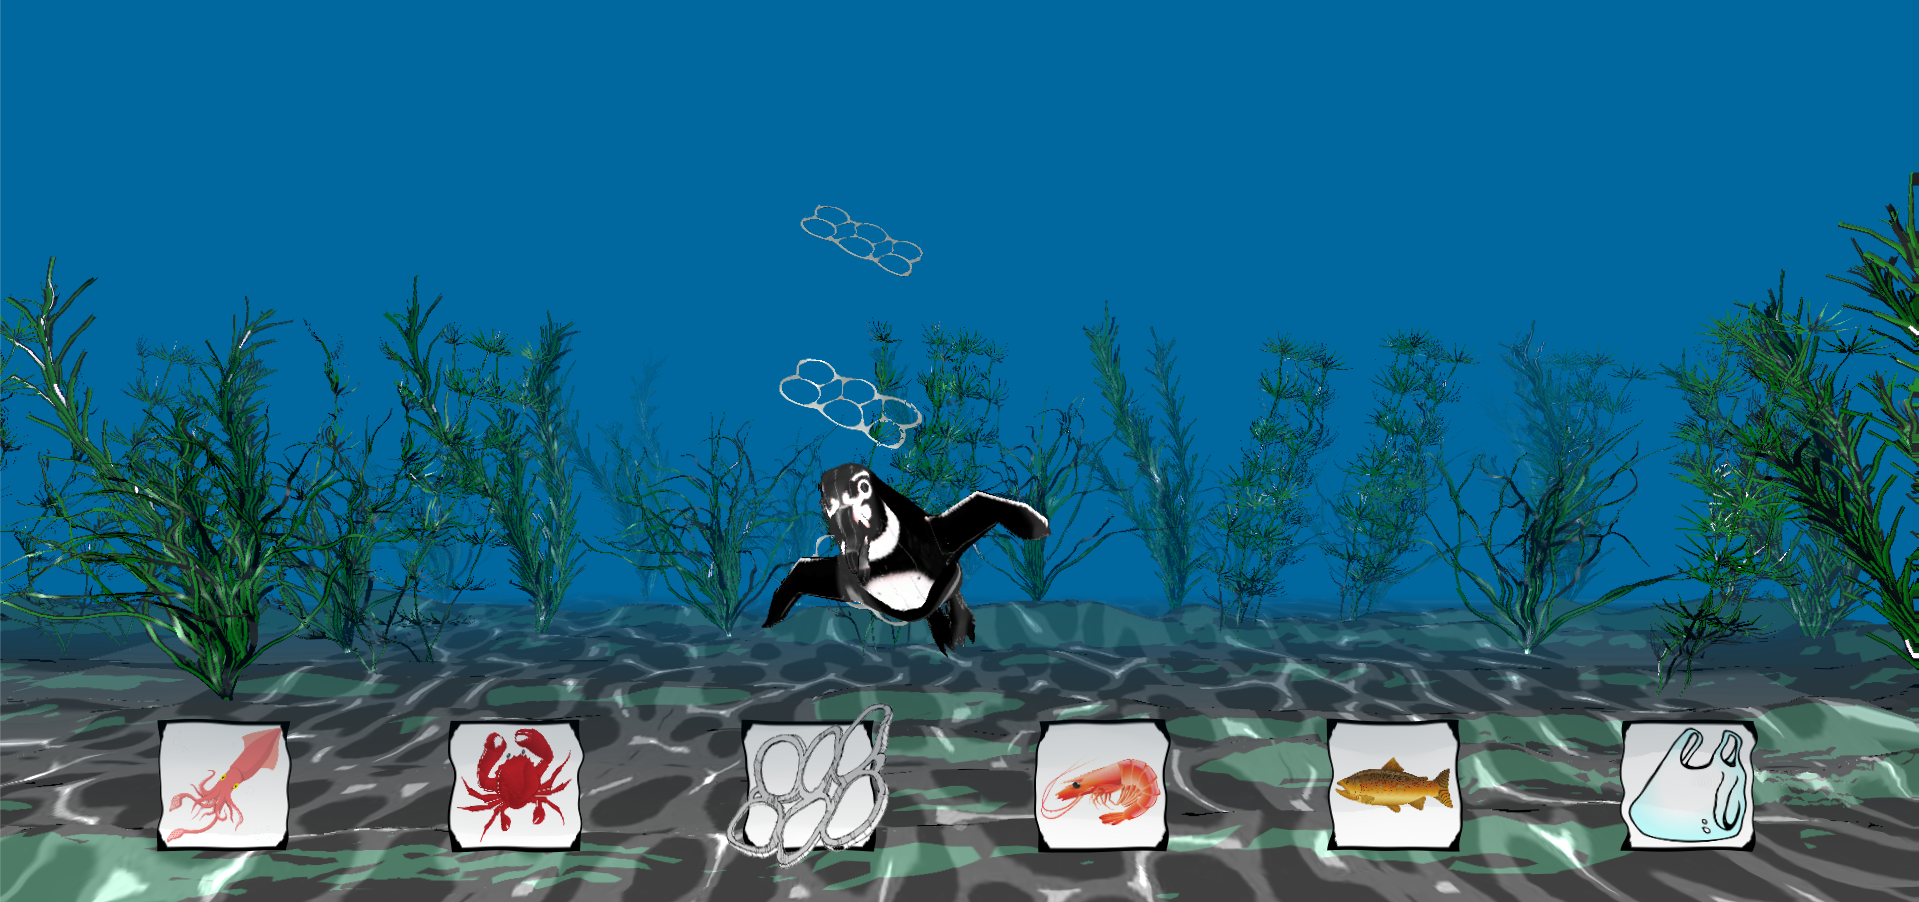
\includegraphics[width=0.9\linewidth]{figure/Design/prototype1FeedAPenguin.png}
	\caption{Screenshot of the \textit{Feed a penguin} prototype. Based on users location on the x-axis the corresponding food item or object in the below icons will spawn and the penguin will eat it if it likes it.}
	\label{fig:prototypeGamified}
\end{figure}

\subsection{Infographically driven experience concept - \textit{Penguin X-Ray}}
\begin{figure}[H]
	\centering
	
\includegraphics[width=0.8\linewidth]{figure/placeholder.png}
	\caption{}
	\label{fig:prototypeInfographic}
\end{figure}

\subsection{Indirectly informative experience concept - \textit{Be a Penguin}}
\begin{figure}[H]
	\centering
	
\includegraphics[width=0.8\linewidth]{figure/placeholder.png}
	\caption{}
	\label{fig:prototypeIndirectInform}
\end{figure}



\section{Implementation}\label{sec:prod1prototypes}
To create the three design prototypes in a low-fidelity manner, it was decided to create them using Unity 2018. Multiple 3D models designed in different modeling software, was used in the implementation as well. Furthermore, the Kinect V2 was used in the first production as well, which translates to being used in all three concepts. The initial Kinect implementation was created following a tutorial\footnote{Kinect tutorial: \url{https://www.youtube.com/watch?v=B7T0XTNk-Vg&index=2&list=PLmc6GPFDyfw-gF4aGw4Etgo0hJSWQcrYQ}}. This code was the baseline of all three concepts, and was utilized in different ways to match the given concept. The original code is created to track head positions and show them as spheres on a canvas. How this is utilized will be explained in the different concepts' chapters. 

The script for the Kinect tracks head locations, and creates a sphere for each location. The Kinect tracks the xyz position of the head, and shows on the canvas where it is located.

\subsection{Penguin X-Ray Concept}
This concept is based on being able to see the skeleton of a penguin through a textured mesh of a penguin. Initially this was done using a Mask created in Unity together with a PNG picture of a penguin skeleton. The mask would track the mouse position and show the picture within the mask on top of the penguin. As seen in \autoref{fig:IP} the mask tracks the position of the head, and shows the PNG in front of the mesh.

\begin{figure}[H]
	\centering
	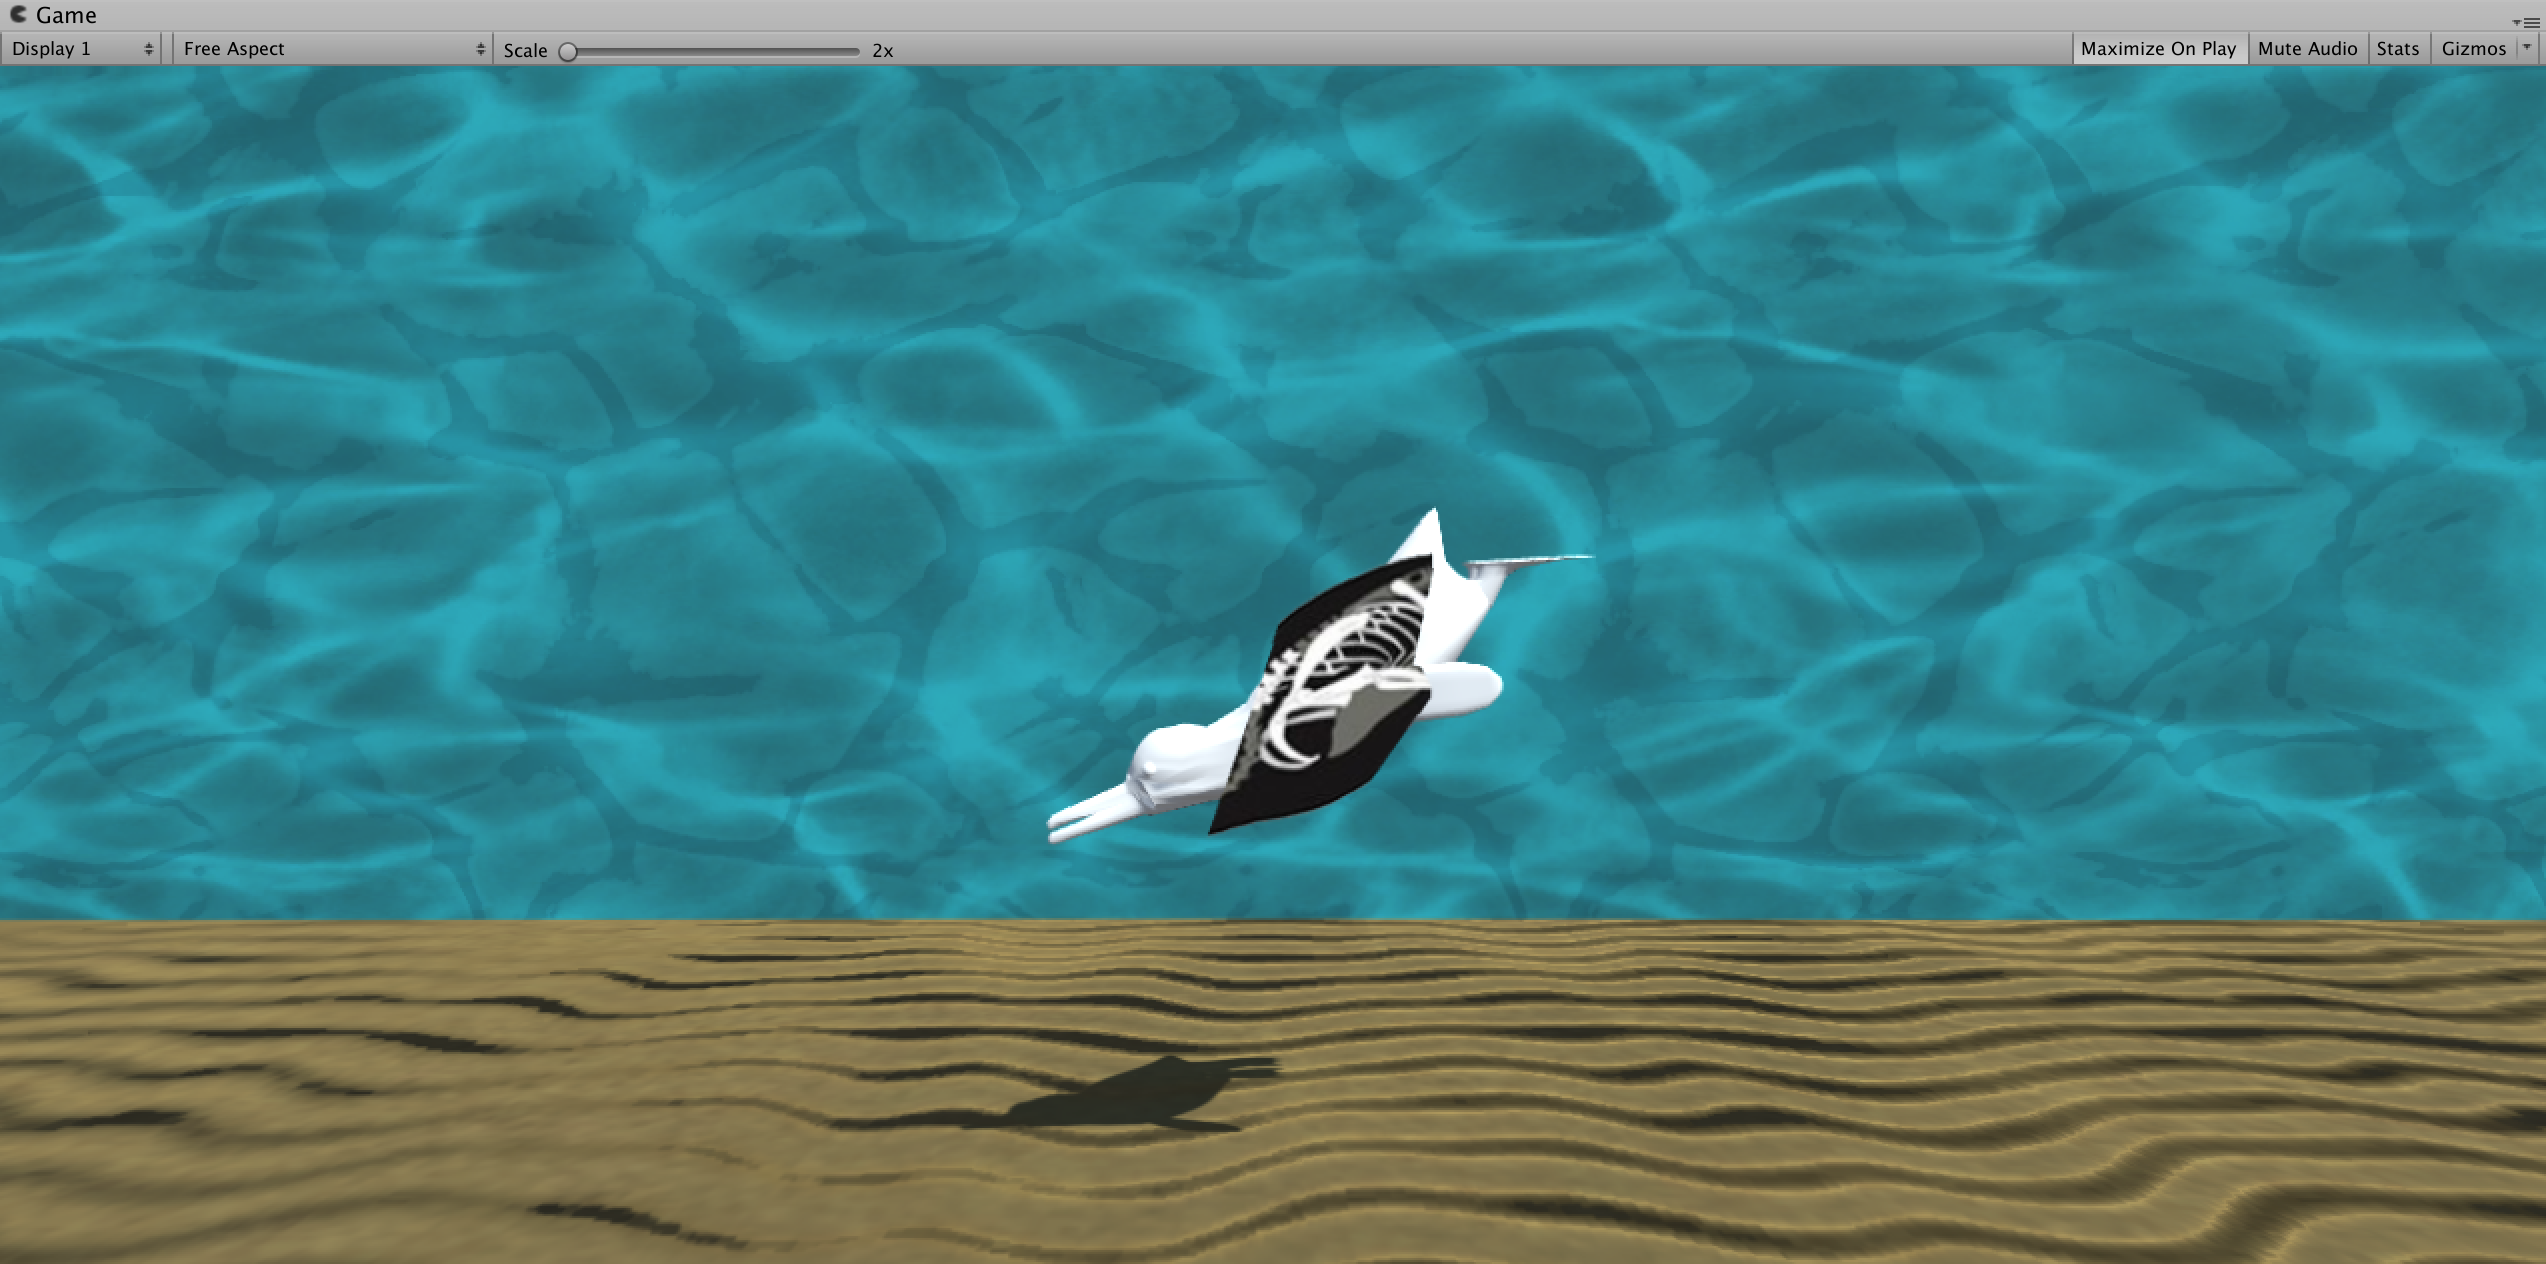
\includegraphics[width=0.9\linewidth]{figure/Implementation/InitialPenguin.png}
	\caption{A picture of the initial early concept}
	\label{fig:IP}
\end{figure}

To build further onto the concept, a real 3D skeleton was used and put inside the penguin. The mask was then used together with the Kinect head tracker, and built into a shader. The head tracker tracks all three axis, but this concept only utilizes the x-axis. The shader with the mask follows the x location of the head tracker. The shader implements a toon shader which is described above. In the shader, the code simply takes points and changes the color to create an x-ray effect. In code snippet \autoref{listing:xrp} 

\begin{listing}[H]
	\caption{}
	\label{listing:xrp}
	\begin{minted}[frame=lines,framesep=2mm,baselinestretch=1.1,fontsize=\footnotesize,linenos]{cpp}
    _DarkColour("Dark colours of XRay", Color) = (0,0,0,.2)
     if(input.position_in_world_space.x > _Point1.x - _PointXSize&& input.position_in_world_space.x 
     < _Point1.x + _PointXSize)
     return _DarkColour;

	\end{minted}
\end{listing}

\subsection{Feed a Penguin Concept}

\subsection{Be a Penguin Concept}



\section{Testing production 1}
To get an understanding of the weaknesses and strengths of each concept, the designs should be tested in multiple iterations. \ 
Firstly, a number of experiments should consider if the technology of the designs is functioning in a such way, that it can be presented to a group of users. Possible problematic findings should be corrected and the designs should be retested until acceptable. A list of criteria is described below in \ref{techExP1}\\
Secondly the three concepts should be presented to a group of test participants from within the target group, namely children. This test should be conducted to obtain an understanding of the interests of target group. This knowledge should be used to develop a final design concept. 

\subsection{Technical experiments}\label{techExP1}
This series of experiments is, as described above, conduced to ensure, that the technologies of the three concepts, is working to the degree of them being presentable for the target group on a level to which they can provide feedback. This feedback should be related to their interest in the concepts. To established when this "degree of working" can be considered acceptable, a list of criteria was created. 

\begin{itemize}
    \item The setup should allow both adults and children to use the interface. 
       \item Each concept should allow minimum four users at a time. As the following testing will be conducted on a group of users rather than individuals, supporting multiple users is necessary.
    \item Each concept should function such that the interactions begins and ends as the user enters and leaves the area of use, respectively. As so, avatars, activated fields and elements, and the alike should activate and deactivate along with the corresponding user. 
    \item All elements designed to be activated or interacted with, must react as intended, and be consistent.  
    \item Each concepts program should live up to the listed criteria for at least 10 minutes after the program has been started.
\end{itemize}

On the location of testing the following user test, another criteria must be taking into account. 
\begin{itemize}
    \item 
 \item The Kinect and interface (being a projector or a screen) should be placed in such manner, that it does not interfere with the use of the interface. For example should a projection consider the users shadow, so that it does not conflict with the interface. \\ 
\end{itemize}

If these listed criteria is achieved, the concepts is considered acceptable for presenting and use in a user test. 

\subsubsection{Results of the technical Experiments} 
The three concepts was evaluated in relation to the listed criteria on a screen within the SMILE-LAb at Aalborg University Copenhagen. 


\subsection{User testing - Focus: The Users interest}

The test participants tried the 3 prototypes explained in \autoref{sec:prod1prototypes}. The goal of the test was to establish how the target group felt about the prototypes, specifically if they found them fun. 

\subsection{Methods}
The following section explains the theoretical framework used, to gather and evaluate data from the test conducted with the target group on the 3 prototypes.   
\subsubsection{Sampling}
Non-probability Sampling: Quota sampling.\\
The test will be conducted on children, as the children are the primary target group for the product. Quota sampling allows the gathering of test participants based on set criteria, such as age. \cite{bjoernerBog}

\subsubsection{Observation}
Direct non-participant observation:\\
This way, it is possible to look straight at the technical faults of the product and see if the interactions work as intended.\cite{bjoernerBog}

\subsubsection{Interview}
Unstructured Interview:\\
As the test participants are children, the unstructured interview is used. This allows the children to have a their thoughts flowing free, while the testers control the topic.\cite{bjoernerBog}

\subsubsection{Reviewing the data}
Review data: Traditional coding.\\
Step 1. Organize\\
Transcribe, catalogue etc to prepare data.

Step 2. Recognize\\
Look at the data multiple times. Find topics, events, themes and concepts that are important to the topic being researched.

Step 3. Coding\\
Label the data under headlines, such as: Major points (Urgent or mentioned several times), unique points(unique thoughts), residual points(the rest of the points found)\cite{bjoernerBog}.

\subsection{Test setup}
One tester hosts the test. The host will maintain all communication with the testers during test!
This tester will introduce the test using the script found in appendix one. This tester will also interview the testers after the test is done. The interview topics are found in appendix one as well. It will be the testers responsibility to ensure that the testers have a close-to-equal introduction to the products as well as have their questions answered during the test. 

The observers will be divided in two different groups:

(1-2) The first observing group will observe if the technical aspects of the test works as intended. The key points they will observe for:\\

Highlight the technical issues found in the test in key words.
Did technical issues affect the test? How?

(1-2) The second observing group will observe on the testers, with a focus on the goal of the test: Do they find the concepts fun?
The observers will write keywords that highlight their experience, through the words they express, their facial expressions and their answers to the interview by the end of the test. The testers does not need to transcribe the full interview, but write key words, both positive and negative. These words will be sorted in a Coding analysis in evaluation.

\subsection{Test results}
% Please add the following required packages to your document preamble:
% \usepackage[table,xcdraw]{xcolor}
% If you use beamer only pass "xcolor=table" option, i.e. \documentclass[xcolor=table]{beamer}
\begin{table}[H]
\label{table:prod1test}
\begin{tabular}{llll}
\rowcolor[HTML]{FFFFFF} 
                                                                         & \textbf{Be a penguin}                                                        & \textbf{Feed a penguin}                                                               & \textbf{Penguin X-ray}                                                         \\
\rowcolor[HTML]{EFEFEF} 
\textbf{Positive:}                                                       & Intuitive interaction                                                        & \begin{tabular}[c]{@{}l@{}}Learning is \\ good and clear\end{tabular}                 & A lot to learn                                                                 \\
\rowcolor[HTML]{FFFFFF} 
                                                                         & Learning about habitat                                                       &                                                                                       & \begin{tabular}[c]{@{}l@{}}Could be used in \\ school contexts\end{tabular}    \\
\rowcolor[HTML]{EFEFEF} 
                                                                         & Good movement                                                                &                                                                                       &                                                                                \\
\rowcolor[HTML]{FFFFFF} 
                                                                         & Fun                                                                          &                                                                                       &                                                                                \\
\rowcolor[HTML]{FFFFFF} 
                                                                         &                                                                              &                                                                                       &                                                                                \\
\rowcolor[HTML]{EFEFEF} 
\textbf{Negative:}                                                       & \begin{tabular}[c]{@{}l@{}}Baby/Adult not \\ understood correct\end{tabular} & \begin{tabular}[c]{@{}l@{}}Felt detached from \\ the interaction\end{tabular}         & \begin{tabular}[c]{@{}l@{}}Found the \\ prototype boring\end{tabular}          \\
\rowcolor[HTML]{FFFFFF} 
                                                                         &                                                                              & \begin{tabular}[c]{@{}l@{}}Took too long \\ to understand \\ the concept\end{tabular} & \begin{tabular}[c]{@{}l@{}}Stopped using the \\ prototype fast\end{tabular}    \\
\rowcolor[HTML]{EFEFEF} 
                                                                         &                                                                              & \begin{tabular}[c]{@{}l@{}}Lost track \\ of themselves\end{tabular}                   &                                                                                \\
\rowcolor[HTML]{FFFFFF} 
                                                                         &                                                                              & Clearer feedback                                                                      &                                                                                \\
\rowcolor[HTML]{FFFFFF} 
                                                                         &                                                                              &                                                                                       &                                                                                \\
\rowcolor[HTML]{EFEFEF} 
\textbf{Tech:}                                                           & \begin{tabular}[c]{@{}l@{}}Lose track when \\ too close\end{tabular}         & \begin{tabular}[c]{@{}l@{}}Bad when close \\ to each other\end{tabular}               &                                                                                \\
\rowcolor[HTML]{FFFFFF} 
                                                                         &                                                                              & \begin{tabular}[c]{@{}l@{}}Dont know \\ plastic 6-pack\end{tabular}                   &                                                                                \\
\rowcolor[HTML]{FFFFFF} 
                                                                         &                                                                              &                                                                                       &                                                                                \\
\rowcolor[HTML]{EFEFEF} 
\textbf{\begin{tabular}[c]{@{}l@{}}Further \\ development:\end{tabular}} & Became an egg                                                                & \begin{tabular}[c]{@{}l@{}}Indicator for \\ where to stand\end{tabular}               & \begin{tabular}[c]{@{}l@{}}Show heart \\ (Generally show \\ more)\end{tabular} \\
\rowcolor[HTML]{FFFFFF} 
                                                                         & \begin{tabular}[c]{@{}l@{}}Indicator for \\ where to stand\end{tabular}      & \begin{tabular}[c]{@{}l@{}}Feed them in a \\ different way\end{tabular}               & \begin{tabular}[c]{@{}l@{}}Indicator for \\ where to stand\end{tabular}        \\
\rowcolor[HTML]{EFEFEF} 
                                                                         & Sounds                                                                       & Sounds                                                                                & Zoom function                                                                  \\
\rowcolor[HTML]{FFFFFF} 
                                                                         & Realistic scenery                                                            & \begin{tabular}[c]{@{}l@{}}Consequence for \\ wrong food\end{tabular}                 & Sounds                                                                        
\end{tabular}
\caption{Table showing the feedback from the Production 1 test}
\end{table}


The table shows the feedback gathered from the test. The feedback given to Be-a-penguin stands out, as the amount of positive feedback was significant compared to the remaining prototypes. The testers found Be-a-penguin fun, as the interaction was subtle, yet easy to realize. It was fun to move around while learning about the habitat and look of the penguins.\\

The test was created to find out which prototypes was the most fun to use for the target group, and thus select this prototype for further development. To establish this, on top of the feedback, a vote was held by the end of the test, where each participant had to choose the prototype they found the most fun. The feedback was as follows:\\

\textbf{Be-a-penguin}: 4 votes.\\
\textbf{Feed-a-penguin}: 1 vote.\\
\textbf{Penguin X-ray}: 1 vote.\\

This establishes that Be-a-penguin will be the concept chosen for further development.
